\section{Durchführung}
\label{sec:Durchführung}

\subsection{Vorbereitungsaufgaben}
\label{sec:vorbereitung}
In folgender Tabelle sind die recherchierten Werte für den Brechungsindex verschiedener Materialien zusammengefasst:
\begin{table}[H]
  \centering
  \caption{Brechungsindizes verschiedener Materialien. \cite{AP02}}
  \label{tab:brechungsind}
  \sisetup{table-format=1.8}
  \begin{tabular}{S S}
    \toprule
    {Material} & {$n$} \\
    \midrule
    {Luft}            & 1.00029317 \\
    {Wasser}          & 1.344661 \\
    {Borkron K1}      & 1.51201 \\
    {Schwerkron SK1}  & 1.61282 \\
    {Plexiglas}       & 1.4931 \\
    {Diamant}         & 2.4235 \\
    \bottomrule
  \end{tabular}
\end{table}

\noindent
Die berechneten Gitterkonstanten werden im Folgenden angegeben:
\\\\
Für $600$ Linien/$\si{\milli\meter}$ gilt
\begin{equation*}
  d = \frac{1}{600} \si{\milli\meter} = \frac{5}{3} \si{\nano\metre}.
\end{equation*}
\noindent
Für $300$ Linien/$\si{\milli\meter}$ gilt
\begin{equation*}
  d = \frac{1}{300} \si{\milli\meter} = \frac{10}{3} \si{\nano\metre}.
\end{equation*}
\noindent
Für $100$ Linien/$\si{\milli\meter}$ gilt
\begin{equation*}
  d = \frac{1}{100} \si{\milli\meter} = \SI{10}{\nano\metre}.
\end{equation*}

\subsection{Versuchsaufbau}
\label{sec:aufbau}
Der Versuchsaufbau besteht aus einer transparenten Platte, auf welcher sich ein roter
($\lambda=\SI{635}{\nano\metre}$) und ein grüner ($\lambda=\SI{532}{\nano\metre}$) Laser
befinden. Die Laser lassen sich dabei im Halbkreis um die Platte bewegen, sodass verschiedene
Winkel eingestellt werden können. Diese können dann an der Skala auf der Platte abgelesen werden.
Um die Experimentierenden vor dem Laserlicht zu schützen, ist zudem noch ein Reflexionsschirm
verbaut. Diese Apparatur ist in Abbildung \ref{fig:Aufbau} dargestellt.
\\\noindent
In der Mitte der Apparatur \ref{fig:Aufbau} lassen sich nun optische Elemente positionieren, welche
in Abbildung \ref{fig:Teile} dargestellt sind.
%
%\begin{figure}[H]
%    \centering
%    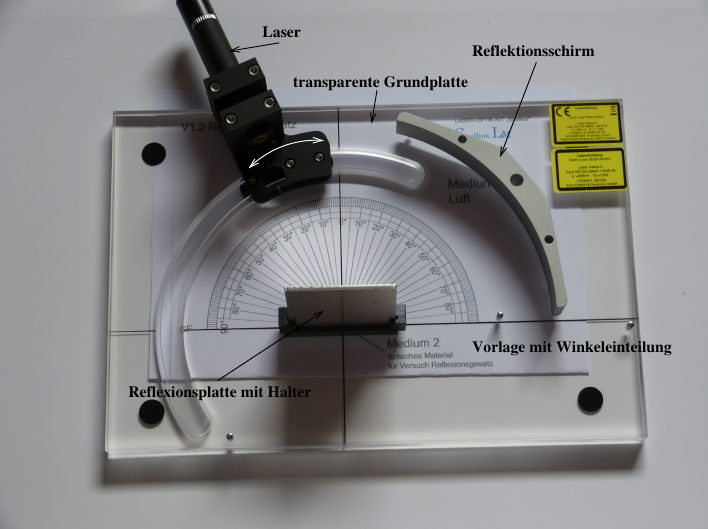
\includegraphics[scale = 0.5]{pictures/Aufbau.png}
%    \caption{Die Versuchsapparatur. Quelle: \cite{AP01}}
%    \label{fig:Aufbau}
%\end{figure}
%\begin{figure}[H]
%    \centering
%    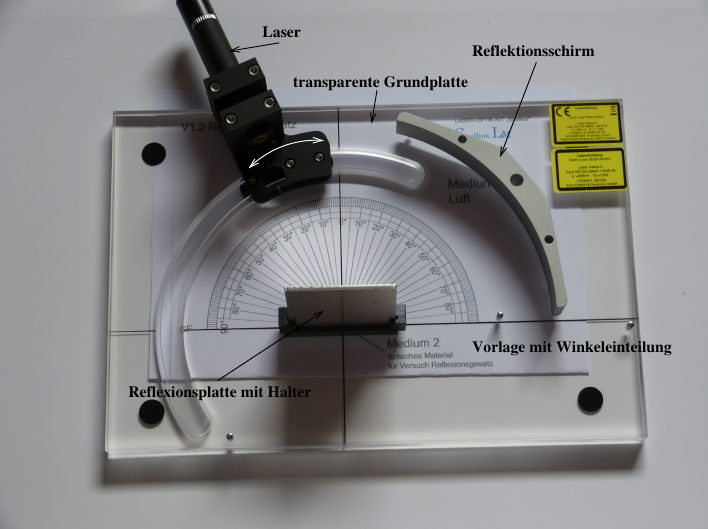
\includegraphics[scale = 0.5]{pictures/Teile.png}
%    \caption{Optische Elemente. Quelle: \cite{AP01}}
%    \label{fig:Teile}
%\end{figure}
%
\begin{figure}[H]
  \begin{minipage}[b]{.55\linewidth} % [b] => Ausrichtung an \caption
     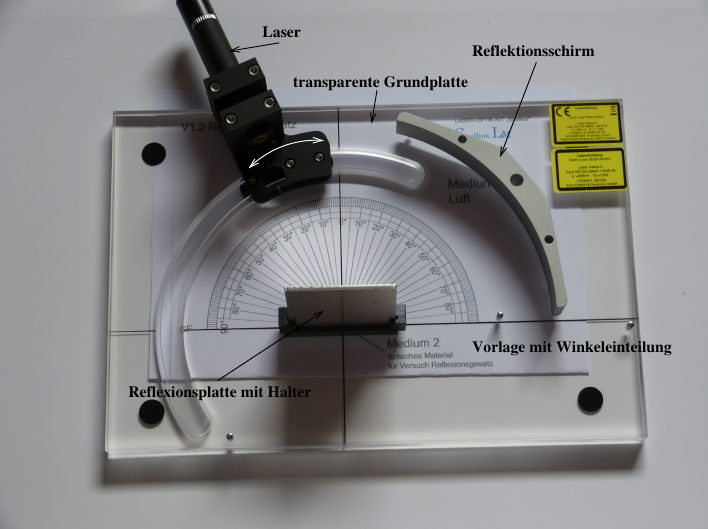
\includegraphics[width=\linewidth]{pictures/Aufbau.png}
     \caption{Die Versuchsapparatur. \cite{AP01}}
     \label{fig:Aufbau}
  \end{minipage}
  %\hspace{.1\linewidth}% Abstand zwischen Bilder
  \begin{minipage}[b]{.55\linewidth} % [b] => Ausrichtung an \caption
     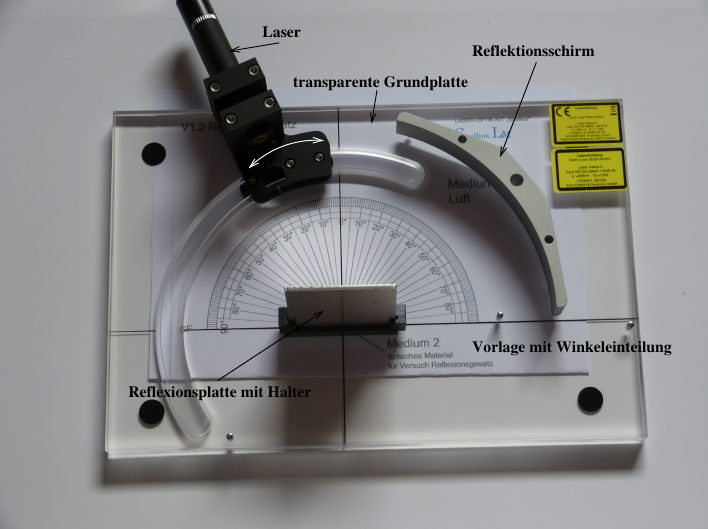
\includegraphics[width=\linewidth]{pictures/Teile.png}
     \caption{Optische Elemente. \cite{AP01}}
     \label{fig:Teile}
  \end{minipage}
\end{figure}

\subsection{Reflexionsgesetz}
\label{sec:reflexionsmessung}
Zur Überprüfung des Reflexionsgesetzes \eqref{eqn:reflexion} wird der grüne Laser an einem Spiel reflektiert. Es wird dabei für
sieben verschiedene Einfallswinkel der Reflexionswinkel notiert.

\subsection{Brechungsgesetz}
\label{sec:brechungmessung}
Das Brechungsgesetz \eqref{eqn:brechung2} für die Näherung $n_{Luft}\approx1$ wird mittels eines Lasers und planparalleler Platte
verifiziert. Dabei wird der grüne Laser auf die planparallele Platte gerichtet. Hinter der Platte wird der Winkel des ausflallenden
Strahls gemessen. Diese Messung wird für sieben verschiedene Einfallswinkel durchgeführt.

\subsection{Planparallele Platten}
\label{sec:planplattemessung}
Mit dem gleichen Versuchsaufbau wie zuvor in \ref{sec:brechungmessung} wird nun der Strahlenversatz von einem Laser durch die
planparallele Platte gemessen. Der Strahlenversatz wird für fünf verschiedene Einfallswinkel gemessen.

\subsection{Prisma}
\label{sec:prismamessung}
Bei diesem Versuch wird in die Mitte der Apparatur ein Prisma aus Kronglas eingesetzt, welches einen brechenden Winkel von
$\gamma=60°$ besitzt. Nun werden sowohl für den grünen, als auch für den roten Laser für fünf verschiedene Einfallswinkel
die Austrittswinkel gemessen. Dabei soll für den Einfallswinkel $10°\leq\alpha_1\leq 60°$ gelten.

\subsection{Beugung am Gitter}
\label{sec:beugungmessung}
Vor der Messung muss der Aufbau justiert werden, sodass der Lichtstrahl den Transmissionsschirm bei $0°$ trifft. Durch die
kreisförmige Anordnung des Transmissionsschirms um die Winkelskala können die Ablenkwinkel $\phi$ direkt abgelesen werden.
Nun werden für verschiedene Gitter die Beugungsmaxima ausgemessen.
Auch bei diesem Versuch werden alle Messungen sowohl mit dem grünen, als auch mit dem roten Laser durchgeführt.
